\documentclass{standalone}
\usepackage{tikz}
\usetikzlibrary{intersections, calc}
\usepackage{hsbcommon}
    \begin{document}
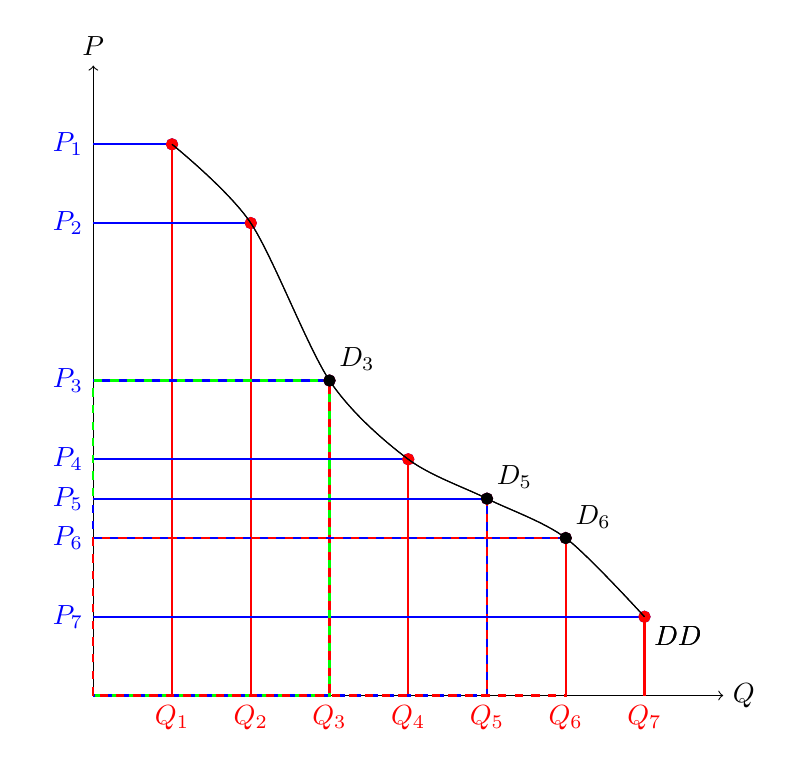
\begin{tikzpicture}
        \draw[->] (0,0) node[below] {\phantom{$X_i$}} -- (8,0) node[right] (Q) {$Q$};
        \draw[->] (0,0) node[left] {\phantom{$Y_mi$}} -- (0,8) node[above] (P) {$P$};

\foreach [count=\i] \demandi in {7,6,4,3,2.5,2,1}{
    \coordinate (C\i) at (\i,\demandi);
    \ifstep{1}{
\begin{scope}[color=blue]

        \filldraw (C\i) circle (2pt);
        \draw[thick] (0, |- C\i ) node[left] {$P_\i$} -- (C\i);
        \draw[dashed] (C\i) -- (C\i |-,0);
    \end{scope}
}

    \ifstep{2}{
\begin{scope}[color=red]

        \filldraw (C\i) circle (2pt);
        \draw[thick] (C\i |-,0) node[below] {$Q_\i$} -- (C\i);
    \end{scope}
}

}

    \ifstep{3}{
\begin{scope}[color=black]

        \draw [name path=demand] plot [smooth] coordinates {(C1) (C2) (C3) (C4) (C5) (C6) (C7)} node[below right]  {$DD$};        
    \end{scope}
}

    \ifstep{4}{

            \draw [name path=demand] plot [smooth] coordinates {(C1) (C2) (C3) (C4) (C5) (C6) (C7)} node[below right]  {$DD$};        
            \foreach \i/\mycolor in {3/green,5/blue,6/red}
            {
                \draw[thick,dashed,color=\mycolor] (0,0) rectangle (C\i);
                \filldraw (C\i) node[above right] {$D_\i$} circle (2pt);
            }

            % \draw[thick,dashed,blue] (0, |- C2) -- (C2) -- (C2 |-,0);
            % \draw[thick,dashed,green] (0,0) rectangle (C3);
            % \draw[thick,dashed,red] (0,0) rectangle (C5);
    }

 

%%% supply curve
        
        % \coordinate (G) at (1,1);
        % \coordinate (H) at (2,3);
        % \coordinate (I) at (3,3.5);
        % \coordinate (J) at (5,4);
        % \coordinate (K) at (6,4.5);
        % \coordinate (L) at (7,7);
        
        % \draw [name path=supply] plot [smooth] coordinates {(G) (H) (I) (J) (K) (L)};
        % \node[right] at (L) {$SS$};
        
        % \path [name intersections={of=demand and supply,by=X}];

        % \filldraw (X) circle (2pt);

        % \draw[dashed, red] (0,0) rectangle (X);
        
    \end{tikzpicture}
\end{document}
